\documentclass{article}

\usepackage[T1]{fontenc}
\usepackage{fancyhdr} % Required for custom headers
\usepackage{lastpage} % Required to determine the last page for the footer
\usepackage{extramarks} % Required for headers and footers
\usepackage[usenames,dvipsnames]{color} % Required for custom colors
\usepackage{graphicx} % Required to insert images
\usepackage{listings} % Required for insertion of code
\usepackage{courier} % Required for the courier font
\usepackage{lipsum} % Used for inserting dummy 'Lorem ipsum' text into the template
\usepackage{hyperref}
\usepackage{color}
\usepackage[normalem]{ulem}
\usepackage{url}

% Margins
\topmargin=-0.45in
\evensidemargin=0in
\oddsidemargin=0in
\textwidth=6.5in
\textheight=9.0in
\headsep=0.25in

\linespread{1.1} % Line spacing

% Set up the header and footer
\pagestyle{fancy}
\lhead{\hmwkAuthorName} % Top left header
\chead{\hmwkClass\ (\hmwkClassInstructor): \hmwkTitle} % Top center head
\rhead{\firstxmark} % Top right header
\lfoot{\lastxmark} % Bottom left footer
\cfoot{} % Bottom center footer
\rfoot{Page\ \thepage\ of\ \protect\pageref{LastPage}} % Bottom right footer
\renewcommand\headrulewidth{0.4pt} % Size of the header rule
\renewcommand\footrulewidth{0.4pt} % Size of the footer rule

\setlength\parindent{0pt} % Removes all indentation from paragraphs

\usepackage{listings}
\usepackage{color}

\definecolor{dkgreen}{rgb}{0,0.6,0}
\definecolor{gray}{rgb}{0.5,0.5,0.5}
\definecolor{mauve}{rgb}{0.58,0,0.82}

\lstset{frame=tb,
  language=Java,
  aboveskip=3mm,
  belowskip=3mm,
  showstringspaces=false,
  columns=flexible,
  basicstyle={\small\ttfamily},
  numbers=none,
  numberstyle=\tiny\color{gray},
  keywordstyle=\color{blue},
  commentstyle=\color{dkgreen},
  stringstyle=\color{mauve},
  breaklines=true,
  breakatwhitespace=true
  tabsize=3
}

\DeclareUrlCommand\ULurl{%
  \renewcommand\UrlFont{\ttfamily\color{blue}}%
  \renewcommand\UrlLeft{\uline\bgroup}%
  \renewcommand\UrlRight{\egroup}}



%----------------------------------------------------------------------------------------
%	DOCUMENT STRUCTURE COMMANDS
%	Skip this unless you know what you're doing
%----------------------------------------------------------------------------------------

% Header and footer for when a page split occurs within a problem environment
\newcommand{\enterProblemHeader}[1]{
\nobreak\extramarks{#1}{#1 continued on next page\ldots}\nobreak
\nobreak\extramarks{#1 (continued)}{#1 continued on next page\ldots}\nobreak
}

% Header and footer for when a page split occurs between problem environments
\newcommand{\exitProblemHeader}[1]{
\nobreak\extramarks{#1 (continued)}{#1 continued on next page\ldots}\nobreak
\nobreak\extramarks{#1}{}\nobreak
}




%----------------------------------------------------------------------------------------
%	NAME AND CLASS SECTION
%----------------------------------------------------------------------------------------

\newcommand{\hmwkTitle}{Eclipse} % Assignment title
\newcommand{\hmwkDueDate}{Marzo 15, 2016} % Due date
\newcommand{\hmwkClass}{Ingegneria del Software 1} % Course/class
\newcommand{\hmwkClassInstructor}{Sr\dj{}an Krsti\'c and Marco Scavuzzo} % Teacher/lecturer
%\newcommand{\hmwkClassTime}{} % Class/lecture time
\newcommand{\hmwkAuthorName}{} % Your name

%----------------------------------------------------------------------------------------
%	TITLE PAGE
%----------------------------------------------------------------------------------------

\title{
\vspace{2in}
\textmd{\textbf{\hmwkClass:\ \hmwkTitle}}\\
\normalsize\vspace{0.1in}\small{Da completare entro \hmwkDueDate}\\
\vspace{0.1in}\large{\textit{\hmwkClassInstructor}}
\vspace{3in}
}

\author{\textbf{\hmwkAuthorName}}
\date{} % Insert date here if you want it to appear below your name

%----------------------------------------------------------------------------------------

\begin{document}

\maketitle

%----------------------------------------------------------------------------------------
%	TABLE OF CONTENTS
%----------------------------------------------------------------------------------------

%\setcounter{tocdepth}{1} % Uncomment this line if you don't want subsections listed in the ToC

\newpage
\tableofcontents
\newpage



%----------------------------------------------------------------------------------------
\section{Introduzione}
\subsection{Java (JRE vs JDK)}
\begin{itemize}
\item \textit{Java Runtime Enviroment} (JRE) \`e un'implementazione della Java Virtual Machine (JVM) che consente di eseguire programmi Java sul vostro calcolatore. Quindi, se la vostra esigenza \`e quella di eseguire delle applicazioni Java, \`e sufficiente la JRE.  
\item  \textit{Java Development Kit} (JDK) \`e necessaria per sviluppare software Java. La JDK contiene al suo interno una o pi\`u JRE oltre a debuggers, compilatori come javac, librerie per lo sviluppo, ecc...
\end{itemize}


\subsection{Eclipse}
\begin{itemize}
\item Eclipse \`e un ambiente di sviluppo (IDE)  \textit{multilinguaggio} e \textit{multipiattaforma} scritto in Java. Un ambiente di sviluppo \` e un software che consente di scrivere altro software. Eclipse \` e multilinguaggio visto che supporta la scrittura di  codice in diversi linguaggi. E' multipiattaforma visto che pu\` o essere eseguito su diverse piattaforme (Linux, Windows, Mac).
\item Eclipse \`e software \textit{open source} i cui autori (pi\`u precisamente i detentori dei diritti) ne permettono e favoriscono il libero studio e l'apporto di modifiche da parte di altri programmatori indipendenti.
\item Pu\`o essere esteso con \textit{plug-in}. Plug-in software che permette l'utilizzo di nuove funzioni non presenti nel software principale.
\end{itemize}





\hrule
\section{Installazione dei tools}
\subsection{Mac OSx}

\textbf{Rimozione della OpenJDK}\\
Per evitare problemi nel corso del progetto si consiglia di rimuovere la OpenJDK se istallata.
\begin{itemize}
\item verifica se e' istallata una JDK: 
\begin{itemize}
\item aprire il terminale
\item digitare \texttt{javac}
\item se ottenete il messaggio command not found andate alla prossima sezione (Installazione Java JDK SE 8u74)
\end{itemize}
\item verifica se una di queste \`e la OpenJDK
\begin{itemize}
\item digitate \texttt{which java javac}
\item se NESSUNO dei path mostrati contengono la sottostringa ``openjdk" andate alla prossima sezione (Installazione Java JDK SE 8u74)
\end{itemize}
\item rimuovi la OpenJDK
\begin{itemize}
\item digita \texttt{sudo rm -rf} percorso della OpenJDK, per esempio\\
 \texttt{sudo rm -rf /Library/Java/JavaVirtualMachines/openjdkx.y.z.jdk}
\end{itemize}
\end{itemize}

\textbf{Installazione Java JDK SE 8u74}
\begin{itemize}
\item connettiti al sito di
  \href{http://www.oracle.com/technetwork/java/javase/downloads/jdk8-downloads-2133151.html}{\ULurl{Oracle}}
\item clicca su ``accept the license agreement''
\item scarica \textit{JDK 8} (SE 8u74) per Mac OS X
\item installa
\end{itemize}

\textbf{Installazione di Eclipse}
\begin{itemize}
\item apri ``applications'' (applicazioni) sul tuo mac
\item crea la cartella ``eclipse''
\item connettiti al sito di \href{https://eclipse.org/downloads/}{\ULurl{Eclipse}}
\item scarica Eclipse Mars.2 (4.5.2) per Mac OS X in particolare Eclipse IDE for Java Developers
\item copia il file scaricato nella cartella ``eclipse'' creata precedentemente
\item estrai il file
\end{itemize}


\subsection{Windows}
\textbf{Installazione Java JDK SE 8u74}
\begin{itemize}
\item connettiti al sito di
  \href{http://www.oracle.com/technetwork/java/javase/downloads/jdk8-downloads-2133151.html}{\ULurl{Oracle}}
\item clicca su ``accept the license agreement''
\item scarica \textit{JDK 8} (SE 8u74) per Windows 
\item scegli correttamente tra Windows x64/x86
\item installa (nota che di default la jre \`e installata sotto ``Program Files/Java'')
\end{itemize}

\textbf{Installazione di Eclipse}
\begin{itemize}
\item apri Program Files (C://Program Files)
\item crea la cartella ``eclipse''
\item connettiti al sito di \href{https://eclipse.org/downloads/}{\ULurl{Eclipse}}
\item scarica Eclipse Mars.2 (4.5.2) per Windows in particolare Eclipse IDE for Java Developers
\item clicca sulla freccia verde rivolta verso il basso
\item clicca su ``open''
\item copia il contenuto della cartella ``eclipse'' nella cartella ``C://Program Files'' precedentemente creata
\end{itemize}

\subsection{Linux (testato con Ubuntu 15.10)}
\textbf{Rimozione della OpenJDK}\\
Per evitare problemi nel corso del progetto si consiglia di rimuovere la OpenJDK se istallata.
\begin{itemize}
\item verifica se e' istallata una JDK: 
\begin{itemize}
\item aprire il terminale
\item digitare \texttt{javac}
\item se ottenete il messaggio command not found andate alla prossima sezione (Installazione Java JDK SE 8u74)
\end{itemize}
\item verifica se una di queste \`e la OpenJDK
\begin{itemize}
\item digitate \texttt{which java javac}
\item se NESSUNO dei path mostrati contengono la sottostringa ``openjdk" andate alla prossima sezione (Installazione Java JDK SE 8u74)
\end{itemize}
\item rimuovi la OpenJDK
\begin{itemize}
\item digita \texttt{sudo rm -rf} percorso della OpenJDK, per esempio\\
 \texttt{sudo rm -rf /Library/Java/JavaVirtualMachines/openjdkx.y.z.jdk}
\end{itemize}
\end{itemize}


\textbf{Installazione Java JDK SE 8u74}
\begin{itemize}
\item apri il terminale
\item  verifica la versione di java con ``\texttt{java -version}''
\begin{itemize}
\item se la versione \`e "1.8.0\_74" hai finito.
\item se no, continua la procedura
\end{itemize}
\item rimuovi openjdk se installato con \texttt{sudo apt-get purge openjdk-*}
\item connettiti al sito di
  \href{http://www.oracle.com/technetwork/java/javase/downloads/jdk8-downloads-2133151.html}{\ULurl{Oracle}}
\item scegli correttamente tra x64/x86 (controlla l'architettura con:  "\texttt{file /sbin/init}")
\item crea la cartella \texttt{sudo mkdir -p /usr/local/java}
\item scegli la cartella dove \`e presente l'archivio, per esempio \texttt{cd /home/"your\_user\_name"/Downloads}
\item copia l'archivio nella cartella di installazione:\\
	\verb!sudo cp jdk-8u74-linux-x64.tar.gz /usr/local/java!
\item scegli la cartella di installazione \texttt{cd /usr/local/java}
%\item rendi eseguibile l'archivio \texttt{sudo chmod a+x jre-8u74-linux-x64.tar.gz}%TODO Are you sure?
\item estraetelo \texttt{sudo tar -zxvf jdk-8u74-linux-x64.tar.gz}
\item Modifica le variabili con \texttt{sudo nano /etc/profile}  e
  aggiungi: \\
\texttt{JAVA\_HOME=/usr/local/java/jdk1.8.0\_74} \\
\texttt{export JAVA\_HOME}\\
\texttt{PATH=\$PATH:\$JAVA\_HOME/bin}\\
\texttt{export PATH}
\item chiudi l'editor (\texttt{ctrl + o} \texttt{enter} \texttt{ctrl + x})
\item applica i nuovi valori (\texttt{source /etc/profile})
\item informa aptitude (apt) della nuova versione di Java installata
\begin{itemize}
\item \verb!sudo update-alternatives --install "/usr/bin/java" "java" \! \\
	  \verb!"/usr/local/java/jdk1.8.0\_74/bin/java" 1!
\item \verb!sudo update-alternatives --install "/usr/bin/javaws" "javaws" \! \\  				      
	  \verb!"/usr/local/java/jdk1.8.0\_74/bin/javaws" 1!
\item \verb!sudo update-alternatives --set java /usr/local/java/jdk1.8.0\_74/bin/java"!
\end{itemize} 
\item verifica la versione \texttt{java -version}
\item riavvia il sistema \texttt{sudo reboot}
\end{itemize}

\textbf{Istallazione di Eclipse}
\begin{itemize}
\item crea la cartella ``eclipse''
\item connettiti al sito di \href{https://eclipse.org/downloads/}{\ULurl{Eclipse}}
\item scegli correttamente tra x64/x86 (controlla l'architettura con:
  "\texttt{file /sbin/init}")
\item scarica Eclipse Mars.2 (4.5.2) per Linux in particolare Eclipse IDE for Java Developers
\item estrailo  \texttt{tar -zxvf eclipse-java-mars-2-linux-gtk-x86\_64.tar.gz}
\item eseguilo \texttt{./eclipse/eclipse \&}
\end{itemize}

%-----------------------------------------------------------------------------------------------------------------

\hrule
\section{Avvia Eclipse}
\begin{itemize}
\item Eclipse non necessita di istallazione. Per eseguire eclipse \` e sufficiente eseguire ``eclipse.exe'' (nella cartella applicazioni o program files a seconda del sistema operativo)
\item Al primo avvio viene chiesto dove salvare il workspace, ovvero la cartella  che conterr\` a tutti i progetti realizzati (\`e possibile modificare il workspace anche in seguito)
\end{itemize}

\begin{itemize}
\item Eclipse all'avvio cerca la JVM del sistema  e setta il Path di default in base a  questa, quindi non \`e necessario  impostare alcun Path per iniziare a  lavorare.
\item Se un progetto dovesse utilizzare una versione della JVM diversa
  da quella di  default \`e necessario modificare il Path del
  progetto:
\begin{enumerate}
\item Clicca Eclipse > Preferences\\
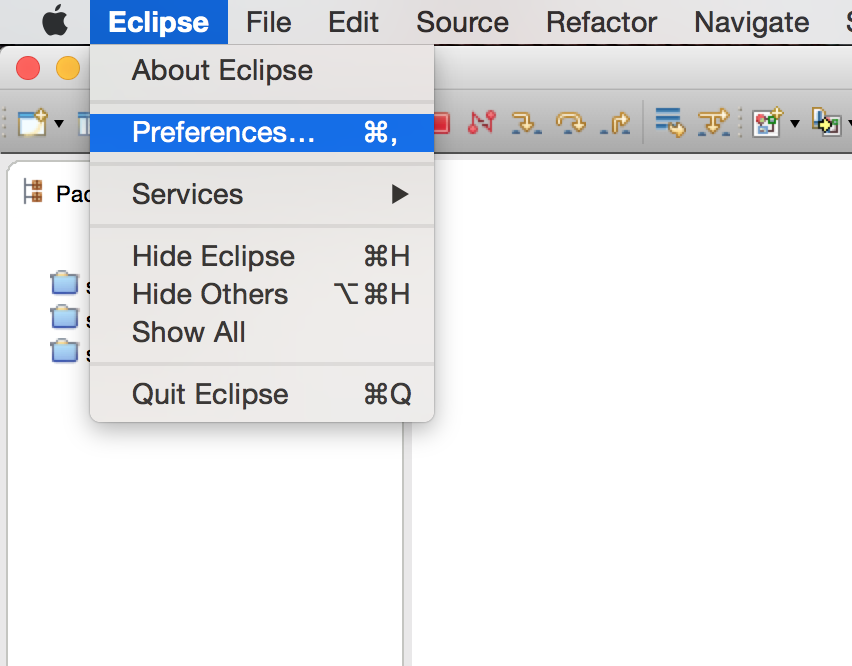
\includegraphics[scale=0.5]{img/01.png}
\item Clicca Java > Installed JREs sulla sinistra\\
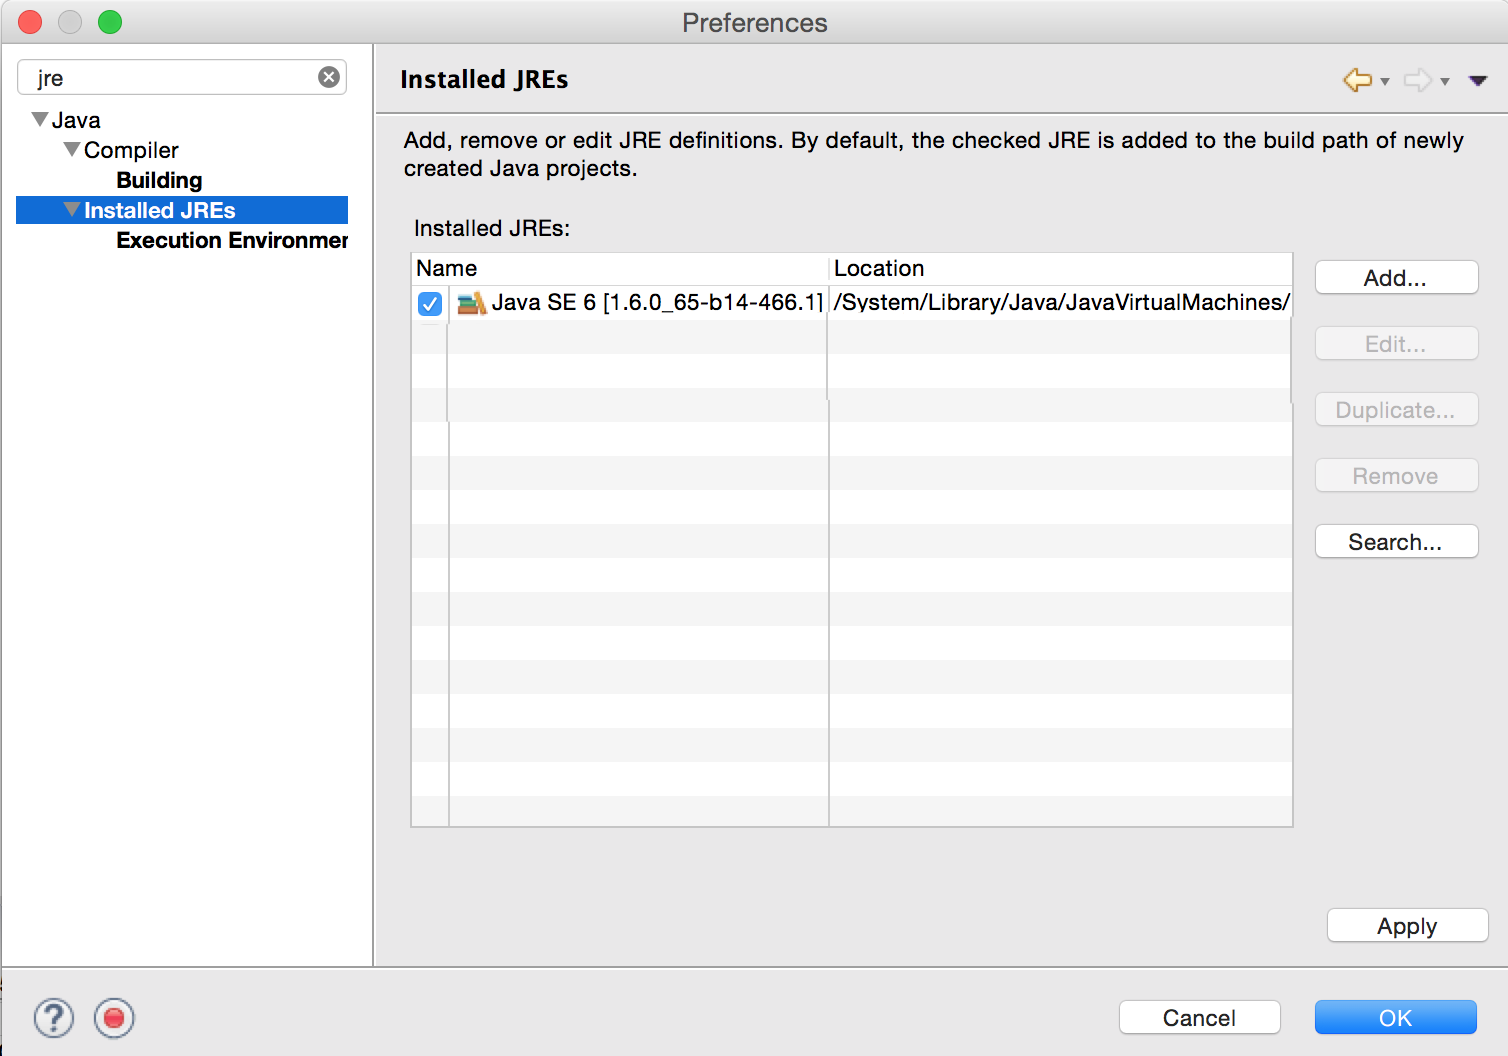
\includegraphics[scale=0.5]{img/02.png}
\item Clicca Add e dopo clicca Directory... e scegli la cartella dove
  ha installato il JDK.\\
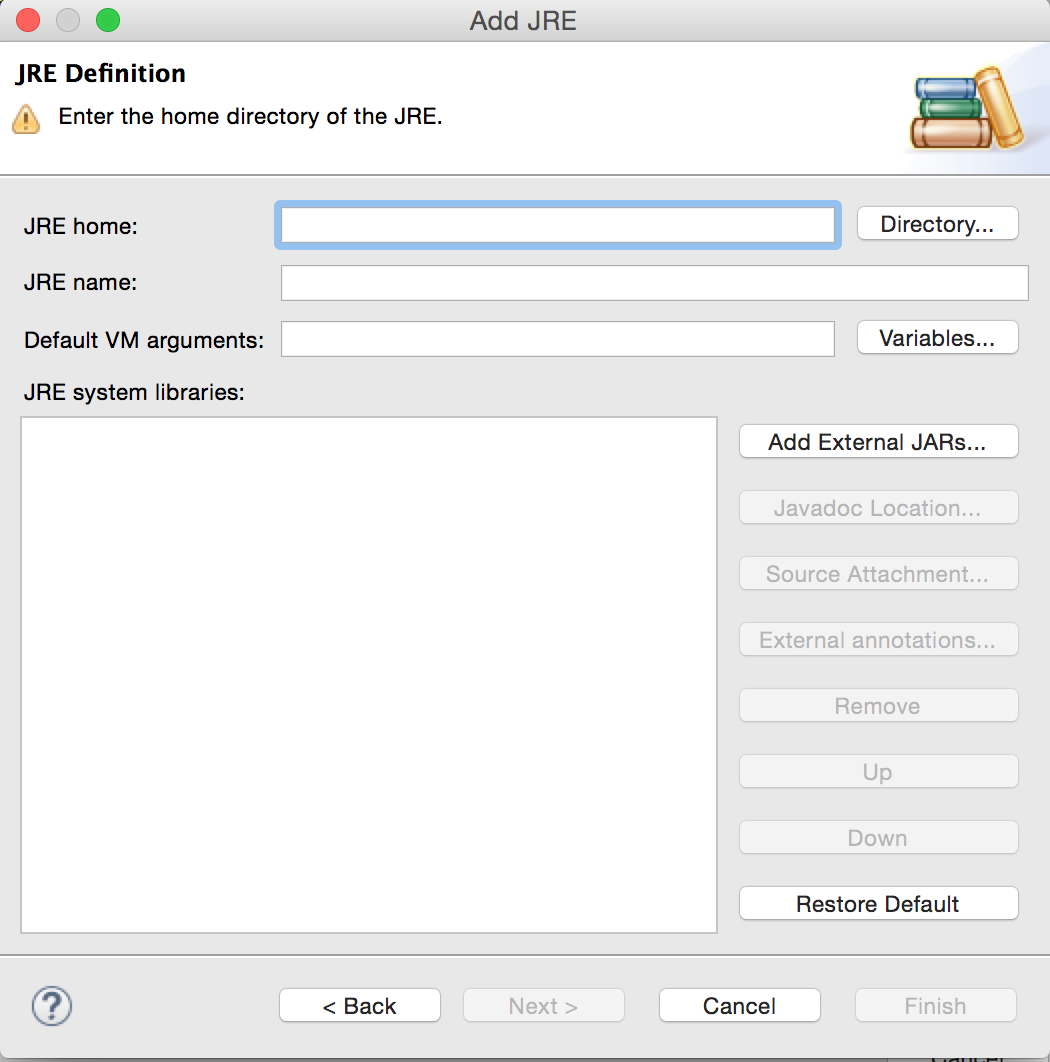
\includegraphics[scale=0.5]{img/03.png}
\item Clicca Finish e Ok\\
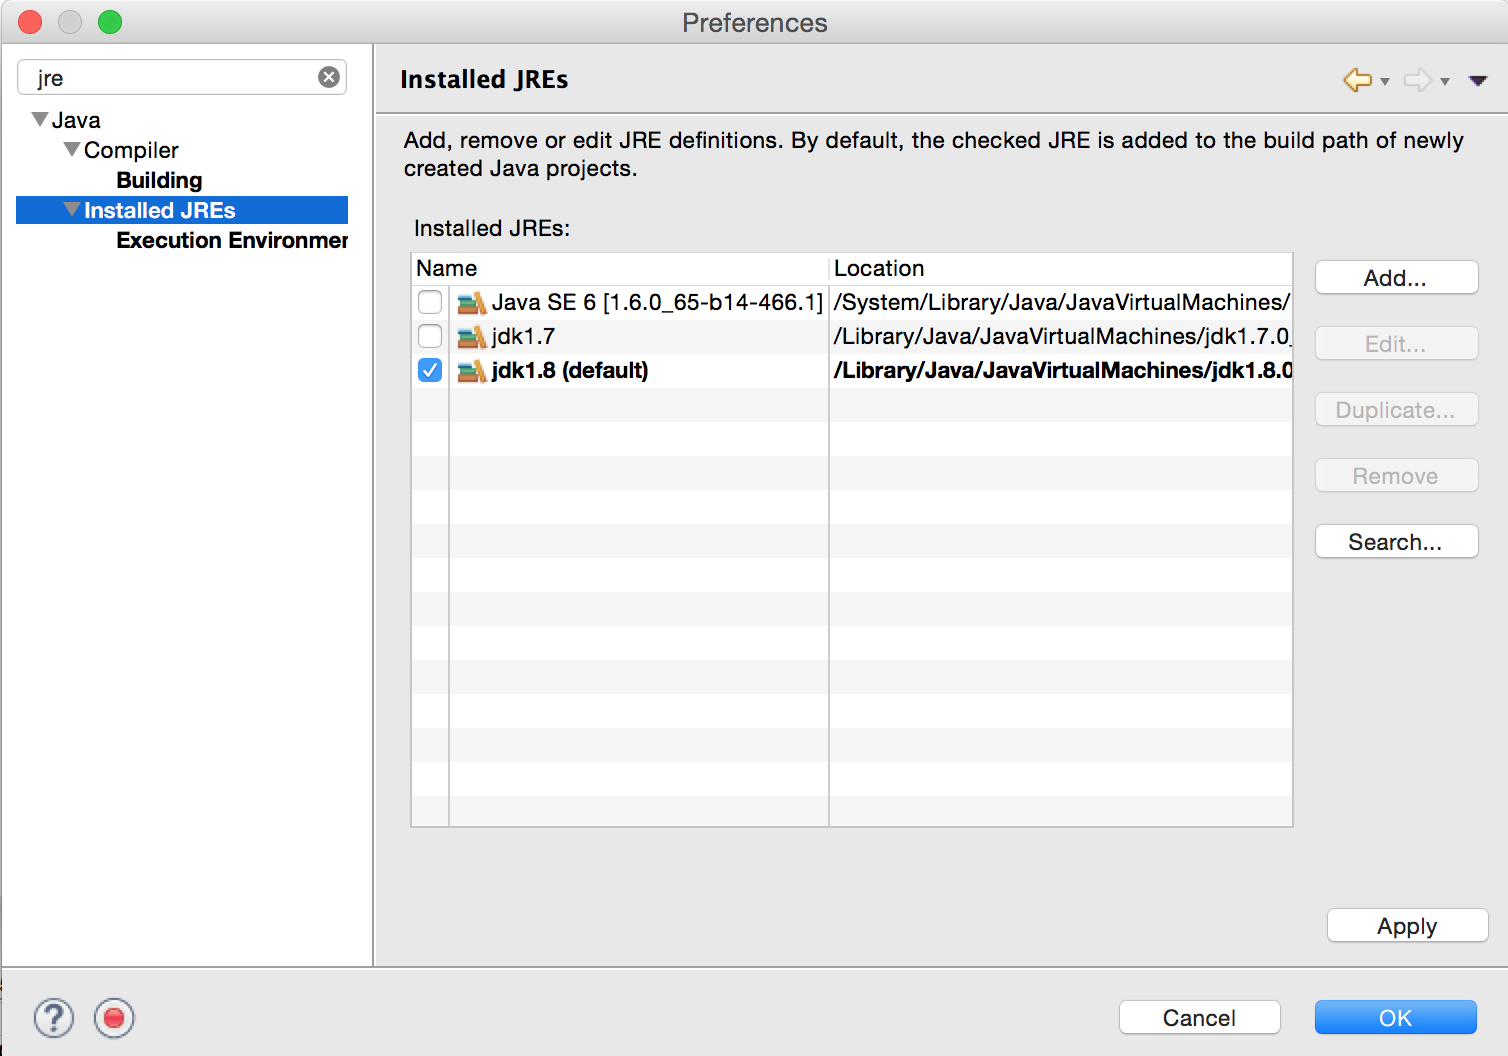
\includegraphics[scale=0.5]{img/04.png}


\end{enumerate}

\end{itemize}
\hrule
\section{Descrizione del Eclipse}

\subsection{Perspectives e Viste}
L'interfaccia grafica di Eclipse \`e organizzata in perspectives. Le perspectives raggruppano diverse funzionalit\'a dell'IDE, per facilitare delle specifiche  operazioni di sviluppo. 
\begin{itemize}
\item La Java perspective ad esempio riunisce strumenti di stesura e organizzazione 
del codice mentre 
\item la Debug perspective fornisce strumenti in fase di debug.
\end{itemize}
Le perspectives sono organizzate in viste. Le viste sono riquadri che offrono supporto per organizzare e scrivere il codice. Per modificare la vista (aggiungere, rimuovere viste) basta andare sotto 
\textit{window} $>$ \textit{show views}


\subsection{La Java perspective}
\begin{itemize}
\item Workspace: cartella che contiene i progetti realizzati
\item Package Explorer: mostra i progetti del workspace, le relative classi e i package 
\item Type Hierarchy View: permette di analizzare la gerarchia di una classe consultandone sotto e super-tipi.
\item Outline: mostra i metodi  implementati e le variabile  definite.
\item Editor: mostra il sorgente dell'applicazione, fornisce funzionalit\` a come per esempio, la gestione del testo (colori), l'assistenza nella scrittura di codice e nella formattazione, nell'inclusione di pacchetti etc.
\item Console: mostra vari tipi di output, tra i quali gli output su console dell'applicazione.
\end{itemize}

% \hrule
% \section{Primi passi con eclipse}
% \subsection{Creare un nuovo Progetto}
% \begin{itemize}
% \item clicca File $>$ New $>$ Project $>$ Java project
% \item scegli il nome del progetto.
% \item clicca Finish.
% \end{itemize}

% \subsection{Creare un nuovo parkage}
% \begin{itemize}
% \item cliccando il tasto destro su src/main/java 
% \item new $>$ package 
% \item scegliere il nome del package 
% \item cliccare Finish
% \end{itemize}
% Il nome di un package \`e generalmente  scelto utilizzando la seguenti regole: 
% \begin{itemize}
% \item  deve contenere solo lettere  minuscole;
% \item deve corrispondere al nome di dominio Internet dell'autore scritto in ordine inverso (it.polimi.ingegneria.software.lab);
% \item deve avere una specificazione dettagliata specie se vi sono pi\`u sottodomini
% \end{itemize}


% \subsection{Creare una nuova Classe}
% \begin{itemize}
% \item click destro sul package (nella vista package explorer)
% \item click su New $>$ Class
% \item inserire nel campo name il nome della classe (Ricorda, il nome delle classi deve inisiare con la lettera maiuscola)
% \item spunta \emph{public static void main} se desideri che il metodo main venga inserito nella classe
% \item eventualmente \`e possibile aggiungere il package della classe.
% \item \`e possibile specificare se la classe \`e  pubblica astratta etc
% \item la classe creata appare all'interno del package explorer e l'editor mostra il codice generato
% \end{itemize}


% \begin{lstlisting}
% package org.sonatype.examples;

% /**
% * Thic class describes a music instument
% * @author the author name
% */
% public class MusicInstrument {
	
% }
% \end{lstlisting}

% \subsection{Aggiungere degli attributi}
% \begin{itemize}
% \item per aggiungere degli attributi \`e sufficiente aggiungere il relativo testo
% \item ricorda, gli attributi iniziano con la lettera minuscola
% \end{itemize}
% \begin{lstlisting}
% package org.sonatype.examples;

% public class MusicInstrument {

% 	/**
% 	 * The musicInstrument's name
% 	 */
% 	private String name;

% 	/**
% 	 * The MusicInstrument's price
% 	 */
% 	private int price;
% }
% \end{lstlisting}

% \subsection{Creare getters and setters}
% \begin{itemize}
% \item click destro sul nome del attributo, Refactor $>$ Encapsulate
%   field...
% \item clicca Ok.
% \end{itemize}

% \begin{lstlisting}
% package org.sonatype.examples;

% public class MusicInstrument {

% 	/**
% 	 * The musicInstrument's name
% 	 */
% 	private String name;

% 	/**
% 	 * The MusicInstrument's price
% 	 */
% 	private int price;
	
% 	/**
% 	 * @return the name
% 	 */
% 	public String getName() {
% 		return name;
% 	}

% 	/**
% 	 * @param name the name to set
% 	 */
% 	public void setName(String name) {
% 		this.name = name;
% 	}
	
% 	/**
% 	 * @return the price
% 	 */
% 	public int getPrice() {
% 		return price;
% 	}
	
% 	/**
% 	 * @param price the price to set
% 	 */
% 	public void setPrice(int price) {
% 		this.price = price;
% 	}	
% }

% \end{lstlisting}


% \subsection{Aggiungere un costruttore}

% \begin{lstlisting}
% public class MusicInstrument {
% 	...
% 	/**
% 	 * Creates a MusicInstrument
% 	 * @param name: is the name of the instrument
% 	 * @param price: price of the instrument
% 	 */
% 	public MusicInstrument(String name, int price)
% 	{
% 		this.name=name;
% 		this.price=price;
% 	}
% }

%  public static void main( String[] args )
%     {
%     	MusicInstrument g1=new MusicInstrument("Charvel", 1000);
%     	MusicInstrument g2=new MusicInstrument("Schecter", 500);
    	
%     	System.out.println(g1.getName());
%     	g1.play();
%     }
% \end{lstlisting}

% \subsection{Istanziare una nuova classe}
% \begin{itemize}
% \item differenza tra dichiarazione e istanziazione
% \item class Guitar
% \item pi\`u istanze del class Guitar
% \end{itemize}


% \begin{lstlisting}
% public class App 
% {
%     public static void main( String[] args )
%     {
%     	MusicInstrument g1=new MusicInstrument("Charvel",1000);
    	
%     	MusicInstrument g2=new MusicInstrument("Schecter", 500);
    	
%     	System.out.println(g1.getName());
%     }
% }
% \end{lstlisting}




% %--------------------------------------------------------------------------------------------------------------------------------------------------------------------------------------------------------
% % METHODS
% %--------------------------------------------------------------------------------------------------------------------------------------------------------------------------------------------------------

% \subsection{Aggiungere un metodo}
% Ricorda, i metodi iniziano con la lettera minuscola

% \begin{lstlisting}
% public class MusicInstrument {
% 	...

% 	/**
% 	 *  plays the instrument
% 	 */
% 	public void play(){
% 		System.out.println("The instrument "+name+" is playing ");
% 	}
% }

% public class App 
% {
%     public static void main( String[] args )
%     {
%     	g1.play();
    	
%     }
% }
% \end{lstlisting}

% \subsection{Overloading}

% \begin{lstlisting}
% /**
% 	 * plays the song
% 	 * @param song: contains the song to be played
% 	 */
% public class MusicInstrument {
% 	...

% 	public void play(String song){
% 		System.out.println("The instrument "+name+" is playing the song: "+song);
% 	}
% }

% public static void main( String[] args )
%     {
%     	MusicIntrument g1=new MusicIntrument("Charvel", 1000);
%     	MusicIntrument g2=new MusicIntrument("Schecter", 500);
    	
%     	System.out.println(g1.getName());
%     	g1.play();
%     	g1.play("Inno alla gioia");
%     }
% \end{lstlisting}

% \subsection{Hierarchy: extends}

% \begin{lstlisting}
% public class Guitar extends MusicInstrument{
	
	
% 	public Guitar(String name, int price) {
% 		super(name, price);
% 	}
% }

% public static void main( String[] args )
%     {
%     	MusicIntrument g1=new MusicIntrument("Charvel", 1000);
%     	MusicIntrument g2=new Guitar("Schecter", 500);
    	
%     	System.out.println(g1.getName());
%     	g1.play();
%     	g1.play("Inno alla gioia");
%     	g2.play("Inno alla gioia");
%      }
% \end{lstlisting}

% \subsection{Aggiungere un attributo e metodi nella sottoclasse}
% \begin{itemize}
% \item Riferimento g2 deve essere il tipo Guitar per chiamare setTuned
%   o isTuned
% \end{itemize}
% \begin{lstlisting}
% public class Guitar extends MusicInstrument{
	
% 	/**
% 	 * Contains the state of the guitar: if it is tuned or not
% 	 */
% 	private boolean tuned;
	
% 	public Guitar(String name, int price) {
% 		super(name, price);
% 		tuned=false;
% 	}
	
% 	/**
% 	 * @return the tuned
% 	 */
% 	public boolean isTuned() {
% 		return tuned;
% 	}

% 	/**
% 	 * @param tuned the tuned to set
% 	 */
% 	public void setTuned(boolean tuned) {
% 		this.tuned = tuned;
% 	}
% }

%  public static void main( String[] args )
%     {
%     	MusicInstrument g1=new MusicInstrument("Charvel", 1000);
%     	Guitar g2=new Guitar("Schecter", 500);
%       	g2.setTuned(true);
        
    	
%     	System.out.println(g1.getName());
%     	g1.play();
%     	g1.play("Inno alla gioia");
%     	g2.play("Inno alla gioia");
%     }
% \end{lstlisting}


% \subsection{Overriding}
% \begin{lstlisting}
% public class Guitar extends MusicInstrument{
% /**
% 	 * Checks if the guitar is tuned and in that case plays the song
% 	 * @param song: contains the song to be played
% 	 */
% 	@Override
% 	public void play(String song){
% 		if(tuned)
% 		{
% 				System.out.println("The instrument "+name+" is playing the song: "+song);
% 		}
% 		else
% 		{
% 			System.out.println("The instrument "+this.getName()+" is not tune, I cannot playing the song: "+song);
% 		}
% 	}
% }
	
% public class App 
% {
%     public static void main( String[] args )
%     {
%     	Guitar g1=new Guitar("Charvel", 1000);
%     	Guitar g2=new Guitar("Schecter", 500);
%       	g2.setTuned(false);
%         g1.setTuned(true);
    	
%     	g1.play("Inno alla gioia");
%     	g2.play("Inno alla gioia");
    	
%     }
% }

% \end{lstlisting}

% \subsection{Utilizzo di super}
% \begin{lstlisting}
% public class Guitar extends MusicInstrument{
% /**
% 	 * Checks if the guitar is tuned and in that case plays the song
% 	 * @param song: contains the song to be played
% 	 */
% 	@Override
% 	public void play(String song){
% 		if(tuned)
% 		{
% 		    super.play(song);
% 		}
% 		else
% 		{
% 			System.out.println("The instrument "+this.getName()+" is not tune, I cannot playing the song: "+song);
% 		}
% 	}
% }
% \end{lstlisting}

% \hrule


% \section{Refactoring del codice}
% Permette di modificare (riscrivere) del codice preservandone il funzionamento (e.g., modificare il nome di una variabile).
% \begin{itemize}
% \item Click destro sulla variabile $>$ Refactor 
% \item Oppure \textit{Alt + Shift + R}
% \end{itemize}

% \hrule
% \section{Gestione di un progetto}
% \subsection{Eseguire un progetto}
% \begin{itemize}
% \item tasto destro sul progetto 
% \item Run as $>$ Run configurations
% \item new Run Configuration 
% \item scegliere il nome
% \item Scegliere Java Application
% \item specificare sotto Main il nome della main class (la classe dove e' contenuto il main)
% \item e' possibile specificare eventuali argomenti utilizzando Arguments 
% \item premere run
% \end{itemize}

% \subsection{Esportare un progetto}
% I progetti in java vengono solitamente esportati come file jar. I file jar sono simili ai file \"zip\".
% \begin{itemize}
% \item nella vista package explorer cliccare con il tasto destro
% \item cliccare su export
% \item cliccare su Jar file (se si desidera creare un file jar contenente il codice dell'applicazione) o su Runnable JAR file se si desidera creare un file jar che puo' essere eseguito (non contiene i sorgenti)
% \item scegliere destinazione e nome del jar file
% \item cliccare su finish
% \end{itemize}

% \subsection{Importare un progetto}
% \begin{itemize}
% \item cliccare su file $>$ import  $>$ existing projects into the workspace  $>$ next 
% \item cliccare su select archive file  $>$  browse e selezionare il percorso del jar
% \item selezionare il progetto da importare
% \item cliccare su finish
% \end{itemize}


 \end{document}

